\cotefile{162-1}

\scanpage{5}
\deleted{Husemöller\qquad Schlessinger, \unsure{functors|functor} of Artin rings.}

\deleted{Mes notes sur cat. de Picard comm.}

\deleted{Saavedra\qquad \unsure{Classes} de Chern des représentations de groupes discrets}

\deleted{Note sur cat. de Picard}

\inserted{\deleted{Notes sur \unsure{gr.|polygr.} de Picard enveloppant d'une cat. triangulée}}

\deleted{\unsure{Rédaction|Réduction} \unsure{prégroupes|polygr. groupes} \illegible{1} en catégorie.}

\noindent$\left\{\begin{array}{l}\text{\deleted{Notes Catégories de Picard}}\\[-1pt]
\text{\deleted{Notes pré-groupes et $\unsure{0^{\mathrm{ième}}|\mathrm O^{\mathrm{ième}}}$ catégorie}}\end{array}\right.$
\margin{\deleted{Notes filtrations et groupes paraboliques}}

Mme Raynaud \quad 1\qquad Papiers de Horrocks

Papier de Popps (?) sur \uline{th.} de Lefschetz\inserted{Zariski} etc pour $\unsure{\pi_1|\pi_r}$

Deligne App. SGA 7 $\overline{\underline{\mathrm{XXI}}}$

Mme Hakim 1\qquad mes notes sur tapis Quillen $\overline{\underline{\mathrm{I}}}\quad\overline{\underline{\mathrm{II}}}$

\deleted{Katz \unsure{'}\qquad notes sur connexions et équations de Picard-Fuchs.}

\deleted{notes sur torsion dans coh. cristalline, et \unsure{sol.} par \unsure{passage|pass.} de \unsure{fnd.|fond.} sur cohomologie évanescente}

\deleted{notes EGA $\overline{\underline{\mathrm{V}}}$}

Verdier 1\qquad \unsure{Prenote|Prenotes} Séminaire Hartshorne

\deleted{\unsure{Singer}\qquad papier Karoubi}

Bardach\qquad \deleted{Thèse Verdier}

Mumford, sur équivalence rationnelle des $0$-cycles

Harder\qquad Sém Bourbaki, avec exposé Deligne

\deleted{Artin : Algebraization of formal moduli $\overline{\underline{\mathrm{I}}},\overline{\underline{\mathrm{II}}}$}

% archive sheet number: 4
\clearpage

\scanpage{6}
Deligne 2 \deleted{(suite)}\qquad \deleted{Compliments Woodshole}

\deleted{\unsure{(Mumford + Matsusaka)|Mumford + Matsusaka)}\quad \unsure{Am. J. Math.|Amer. J. Math.} 1964}

\deleted{Mumford : Abelian quotients of Teichmüller group}

Mumford : Some aspects of the Pb of Moduli (mimeo.)

\deleted{Lang Néron}

\noindent Matsusaka $\left|\begin{array}{l}\text{\unsure{chow|char.} of Jac. variety}\\ \text{A correction to \ldots}\\ \text{The criteri. for alg \unsure{equivalens|equivalence} \unsure{.\,--|\ldots}}\end{array}\right.$

\deleted{Néron : \unsure{Quasi-fonctions|Quasi fonctions} et hauteurs sur les V.A.}

\deleted{Kleiman : notes pour SGA 6}

\deleted{Grothendieck : lettre à Hartshorne du 25.9.67 (sur son papier de dim. coh. des Var alg).}

\(\left.\begin{array}{l}\text{\deleted{Weil}}\\\text{Andreotti}\end{array}\right\vert\ \text{sur Torelli}\)

\deleted{Rédaction \unsure{Mumf|Mumf.} lemme de Abhyankar}

\deleted{Artin\qquad Kiehl, sur th. de Frisch, Inventiones Mathematicae}

\deleted{Samuel\qquad Papiers de Ramanan}

\dashuline{Berthelot} \deleted{(2)} 1 ///\quad Gabriel : \uline{groupes formels}

\deleted{Cartier : notes CR gr. form.}

notes sur stratifications

\deleted{notes sur groupe de BT et Cristaux}

\deleted{Artin\qquad Kiehl Ausgezeichnete Ringe.}

\deleted{Saavedra\qquad Atiyah, \uline{Finiteness} Theorems for compact}

\deleted{Lie groups}

\deleted{\unsure{Dolotheo|Dolontho|Dolotho}\qquad SGA 6 $\underline{\mathrm{X}}$ (\unsure{Manin|Mumford} \unsure{formel})}

\deleted{B. Mazur\qquad Correspondance avec Griffiths}

\deleted{Notes Kleiman, conj. \unsure{standart|standard}}

\deleted{\uline{Deligne} (suite))\qquad Notes \unsure{Jussila|Jussita}}

\deleted{Lettre : \unsure{Oort|Obstruction|O. Zariski} - \unsure{Piatetzki|Piatezki}-Schapiro}

\deleted{Notes CR \deleted{\unsure{Gabriel}} Cartier, groupes formels.}

\deleted{Notes \unsure{Catégories|Catégorie} \unsure{cofibrées|triangulées} \illegible{1}}

\deleted{\uline{Murre}\qquad Conjecture sur \unsure{Rosenlicht} uniforme}

\deleted{SGA 7 $\overline{\underline{\mathrm{I}}}$ \unsure{à|:} $\overline{\underline{\mathrm{V}}}$}

\deleted{Rim\qquad Thèse Gabriel}

Quillen\qquad \deleted{lettres à Verdier :}

Notes Verdier limite projective

Notes Karoubi sur définition de $K$.

% archive sheet number: 5
\clearpage

\scanpage{7}
\uline{Szpiro}

\(\left\Vert\begin{array}{@{}p{.91\linewidth}@{}}Notes de moi et \unsure{Bon|Bou|Bass} sur \unsure{caractérisation|caracterisation} des Gorenstein\\Notes sur $\exists$ complexe dualisant en dim 1\end{array}\right.\)

Notes SGA 7

\deleted{Notes sur dualité de Poincaré en coh. de Hodge des variétés alg. singulières (A) à (E)).}

\deleted{\uline{Hartshorne}\qquad SGA 2}

\deleted{\unsure{R|K} Livre Verdier}

\uline{Balasko}

\deleted{Notes}\quad\(\left\{\begin{array}{l}\text{\deleted{$\underline{NS}_{X/S}\unsure{\mathbin{-\!\circ}|\to}\underline{NS}_{B/S}$ etc}}\\\text{\deleted{produit de convolution sur VA}}\end{array}\right.\)

\deleted{3 Articles de Rim-Buchsbaum}

\deleted{Notes EGA V sur idéaux de Fitting}

\deleted{\uline{Giraud}\qquad Notes Cartier sur vecteurs de Witt.}

\deleted{\uline{Theodoros}}\qquad \deleted{Bourbaki}\ \(\left\{\begin{array}{l}\text{\deleted{Top. Gén. $\overline{\underline{\mathrm I}}$}}\\\text{\deleted{\unsure{Ens|Ets} $\overline{\underline{\mathrm I}}$}}\end{array}\right.\)

Poenaru\qquad Atiyah-Hirzebruch, über Cohomologieoperationen\unsure{-|\ldots} \unsure{---|\ldots}

Stolzenberg : revue livre Bishop \ldots

\deleted{Bardach (suite)\qquad 2 articles d'Artin sur singularités rationnelles}

\deleted{\unsure{Houzel|Housder}\qquad Artin : a) Contractions\quad b) Foncteurs représentables}

Saint Donat 1\qquad SGA 5 $\overline{\underline{\mathrm{IV}}}$ (Notes Jouanolou)

\deleted{SGA 7 $\overline{\underline{\mathrm I}}$ à $\overline{\underline{\mathrm V}}$ (\unsure{1 à|I à|en} \unsure{microfiches|microfilms})}

Livre Mumford VA

Notes Deligne\qquad \(\left\{\begin{array}{@{}p{.67\linewidth}@{}}sur th. de Lefschetz vache\\sur conj pour courbes rel. (cf SGA 4 $\overline{\underline{\mathrm{XVIII}}}$)\end{array}\right.\)

% archive sheet number: 6
\clearpage

\scanpage{8}
\reversemarginpar
Berthelot 2

% slanted
\margin{\uline{redemander}}

\(\left\{\vcenter{\hbox{\begin{minipage}{.89\linewidth}
Deligne \(\left\{\begin{array}{@{}p{.75\linewidth}@{}}\deleted{Structure à l'$\infty$ des \unsure{éqs|éqns} P.F.}\\\deleted{lettre à Leray et Washnitzer}\end{array}\right.\)

Katz\quad \(\left\vert\begin{array}{@{}p{.79\linewidth}@{}}Th. de Dwork (2 papiers)\\Theory of regular singular points\\\unsure{Nilpotence|Nilpotent} connection of Gauss Manin\par\hfill(2 papiers)\\Th. de monodromie \unsure{vs.|v.|cr.} Berthelot\end{array}\right.\)

Grothendieck : Torsion en ch. cristalline.

Petit papier Deligne sur prémorphismes de sites.

Papiers Deligne : Sém Harvard

SGA 5 $\overline{\underline{\unsure{\mathrm{VII}|\mathrm{XII}}}}$ \S\S\ 1,10 (Jouanolou)

Notes Katz connexions intégrables (MA)
\end{minipage}}}\right.\)

Illusie \deleted{\illegible{1}}\qquad lettre à Giraud sur obstructions aux rel. de groupes lisses.

Papier Mazur-Roberts sur char. d'E-P.

% slanted
\margin{\tikz[baseline=(t.base)]{\node[inner sep=1pt] (t) {\deleted{\uline{redemander}}};\draw (t.center) ellipse [x radius=2.6em,y radius=.65em];}}

\deleted{2 \uwave{paquets notes sur opérations de Cartier}}

Notes sur th. de Deligne sur ``torseurs universels''.

\deleted{SGA\deleted{4} 6 $\overline{\underline{\mathrm I}}\ \overline{\underline{\mathrm {II}}}\ \overline{\underline{\mathrm {III}}}$ pour révision}

Serre : variétés qui ne se relèvent pas en \inserted{\uline{car. 0}}

Seydi\qquad Notes sur \unsure{lemme|lemmes} Hironaka

\deleted{Thèse Verdier} sur morphismes univ. ouverts

\uline{Thomas} 1\qquad Papiers \unsure{Lindenstrausss|Lindenstrauss}, Pelczynski etc

Survey de Lindenstrauss \unsure{---|--}

\uline{Jurchescu}\qquad Knorr, Finitude, $\overline{\underline{\mathrm I}}$, $\overline{\underline{\mathrm {II}}}$.

Petit livre sur finitude

Goldschmidt\qquad \unsure{Brieskorn|Brishorn} $\{$singularités rationnelles - - - -$\}$

\deleted{Grauert}\qquad \deleted{Artin, alg. of formal moduli $\overline{\underline{\mathrm I}}$,$\overline{\underline{\mathrm {II}}}$}

% archive sheet number: 7
\clearpage
\normalmarginpar

\scanpage{9}
\deleted{\unsure{Brieskorn|Briskorn}}

\deleted{2 lettres Deligne sur connexions intégr.bles (sur $\mathbb C$)}

\deleted{Notes Serre formes quadratiques}

\deleted{Rapport Griffiths sur périodes}

\deleted{Séminaire Chevalley gr. \unsure{semi|ses} alg.}

\deleted{Schlessinger, \unsure{thèse|Thèse}}

\deleted{Trois tirages \unsure{à} \unsure{part} de Bott}

\deleted{Borel : Springer Lecture Notes}

\deleted{Rim : SGA 7 $\overline{\underline{\unsure{\mathrm{XVI}|\mathrm{VI}}}}$}

Demazure\qquad \deleted{notes sur Kostant, sur résolution d'un morphisme ....}

Saavedra\quad \(\left\{\vcenter{\hbox{\begin{minipage}{.87\linewidth}
\deleted{Griffiths, Schmid}

\deleted{Bourbaki Groupes de Lie}

\deleted{Notes sur polarisations dans catégories tannakiennes}

\deleted{Notes sur structure de Hodge, lettre : Mumford, deriv. transc. des motifs en car. 0}

\deleted{Tate : \uline{cohomologie} tores}
\end{minipage}}}\right.\)

Bitzakis\qquad Bourbaki Algèbre

\deleted{Van de Ven}

\deleted{Mes notes sur}

\deleted{SGA 7 XX (Katz : le th. de Griffiths \unsure{)|\S}}

\deleted{\uline{Griffiths : Report on Variation of Hodge structure}}

Saint Donat 2\qquad \(\left\vert\begin{array}{@{}p{.68\linewidth}@{}}SGA 5 $\overline{\underline{\mathrm{XVIII}}}$\\Notes Mumford sur variétés définies par \unsure{équs.|éqs.} quadratiques\\Livre Mumford V.A.\end{array}\right.\)

Hubbard\qquad \unsure{tir.g.|tir.g} à part sur rigidité des structures complexes (\unsure{Man.|Ann.} Math.)

Nakis\qquad Produits tens. top. (Groth.)

% archive sheet number: 8
\clearpage

\scanpage{10}
\uline{Lascou}\qquad Borel-\unsure{Hirzebruch|Hirzebroch} $\overline{\underline{\mathrm I}}\ \overline{\underline{\mathrm {II}}}$

Borel thèse

Serre \unsure{Gèbres|Gèbrs}

Mazur\qquad Lettre à Serre corps \unsure{classe|class} local etc

\deleted{Notes Katz connexions ``intégrables''}

Quillen : Complex cobordism $+$ formal groups

Lettre de Barsotti

Rim SGA 7 $\overline{\underline{\mathrm{VII}}}$

Teissier\qquad 2 articles \unsure{Brieskorin|Brieskorn} rés. d'un morphisme.

\unsure{Fígeroa|Figeroa}\qquad Article Serre 1957

Fouzat\qquad Article Mumford $0$-cycles

\uline{Saavedra}\qquad \(\left.\begin{array}{@{}p{.58\linewidth}@{}}Groupes ${}^{1}\!/\!{}_{2}$ simples et esp. riem. sym.\\\rule{2em}{.35pt} et Algèbres de Lie\end{array}\right\vert\ \text{Bourbaki}\)

SGA 4 $\overline{\underline{\mathrm{IV}}}$

% archive sheet number: 9
\clearpage

\cotefile{162-6}

\scanpage{2}
\[
\begin{aligned}
\gamma_{\mathbb{R}}(s)&=\pi^{\frac{s}{2}}\,\Gamma\bigl(\tfrac{s}{2}\bigr)\\[4pt]
\gamma_{\mathbb{C}}(s)&=\tfrac{1}{2}\,\deleted{\unsure{\tfrac{1}{2}|2}}\,(2\pi)^{s}\,\Gamma(s)
\end{aligned}
\]
\figure{
\begin{tikzpicture}[x=.75cm,y=.75cm]
\draw[line width=.25pt] (0,0) .. controls (2,.05) and (4.5,.13) .. (6,.04) .. controls (7.5,0) and (9,-.12) .. (10,-.14);
\end{tikzpicture}}

\[
\begin{aligned}
&\begin{aligned}[t]
&\text{\uline{$\mathbb{R}$}}\\[6pt]
&n=2p
\end{aligned}
\quad
\prod_{p<q}\gamma_{\mathbb{C}}(s-p)^{h(p,q)}\cdot
\left\{\begin{array}{@{}l@{\quad}l@{}}
h_{p}^{+}: & F=(-1)^{p}\\
h_{p}^{-}: & F=\deleted{\unsure{(-1)|(1)|(}}-(-1)^{p}\\[2pt]
\multicolumn{2}{@{}l@{}}{\displaystyle {}\cdot\gamma_{\mathbb{R}}(s-p)^{h_{p}^{+}}\,\gamma_{\mathbb{R}}(s-p+1)^{h_{p}^{-}}}
\end{array}\right.
\end{aligned}
\]

\[
\text{\uline{$\mathbb{C}$}}\qquad
\prod_{pq}\gamma_{\mathbb{C}}\bigl(s-\inf(p,q){\bigr)\rlap{\(\unsure{\mathpunct{:}|\mathpunct{.}}\)}}^{h(p,q)}
\]
% archive sheet number: 1
\clearpage

\scanpage{3}
\noindent\uuline{$\unsure{\operatorname{Gal}|\operatorname{gal}}(E/\mathbb{Q})\;-\;C(E)$}

\diagram{\(\displaystyle
\begin{array}{@{}l@{\qquad}c|l@{}}
\text{\uline{$W_{\mathbb{R}}^{\unsure{\prime|\cdot}}$}}: & \sigma & \sigma\unsure{x|u}\sigma^{-1}=\unsure{\bar{x}|\bar{u}}\\[3pt]
\tikz[baseline=(z.base)]{\node[inner sep=1pt] (z) at (0,0) {$\mathbb{Z}/2$};\node[inner sep=1pt] at (1.7,0) {$\mathbb{C}^{*}$};\draw (-.45,-.22) -- (-.45,-.36) .. controls (.3,-.40) and (1.4,-.65) .. (1.94,-.52) .. controls (2.15,-.47) and (2.18,-.41) .. (2.15,-.28);}
& \mathbb{C}^{*} &
\sigma^{2}=\tikz[baseline=(one.base)]{\node[inner sep=1pt] (one) {$-1$};\draw[rotate around={15:(one.center)}] (one.center) ellipse [x radius=1.05em,y radius=.72em];}
\end{array}
\)}
\figure{\begin{tikzpicture}[x=1cm,y=1cm]
\draw[line width=.25pt] (0,.04) .. controls (1.2,-.10) and (2.4,.05) .. (3.3,0) .. controls (5,-.04) and (5.8,-.27) .. (6.8,-.16) .. controls (8,-.08) and (9,-.18) .. (9.7,-.21);
\end{tikzpicture}}

\[
H^{2}(\mathbb{Z}/2,\mathbb{C}^{*})=\text{\uline{$\mathbb{Z}/2$}}
\]

\figure{\begin{tikzpicture}[x=1cm,y=1cm]
\draw[line width=.25pt] (0,0) .. controls (.6,.14) and (1.6,.12) .. (3,.09) .. controls (5,.12) and (7.6,-.03) .. (8.5,-.07) -- (9.6,-.16);
\draw[line width=.18pt] (10.04,-.31) -- (10.52,-.35);
\end{tikzpicture}}
\diagram{\(\displaystyle
\begin{array}{@{}l@{\quad}l@{\,}c@{\,}l@{}}
\begin{array}[t]{@{}l@{}}
M\\[2pt]R\;-\;\text{\uline{$\mathbb{C}$}}
\end{array}
&
\begin{array}[t]{@{}l@{}}
{\deleted{H(\mathbb{C})}}^{(\unsure{p\cdot q|p,q|pq|p:q})}\\[2pt]
H(M(\mathbb{C}),\mathbb{R})
\end{array}
&
\begin{array}[t]{@{}c|c@{}}
\sigma & \sigma\\[5pt]
\deleted{\mathbb{C}^{*}} & S
\end{array}
&
\bigg|\;\sigma^{2}=+1\\[-1pt]
&\multicolumn{2}{c}{\displaystyle
\prod_{\unsure{\mathbb{C}|C}/\unsure{\mathbb{R}|R}}\mathbb{G}_{m}\;=}
&
\end{array}
\)}
% archive sheet number: 2
\clearpage

\scanpage{4}
\diagram{\begin{tikzcd}[ampersand replacement=\&,column sep=1.8em,
execute at end picture={\draw[line width=.25pt] ([xshift=-2pt,yshift=-2pt]dom.south west) -- ([xshift=-2pt,yshift=-5pt]dom.south west) -- ([xshift=2pt,yshift=-5pt]gm.south east) -- ([xshift=2pt,yshift=-2pt]gm.south east);}]
N\unsure{\mathpunct{;}|\mathpunct{:}}\& |[alias=dom]| S_E \arrow[r] \& S_{\mathbb{Q}}\arrow[r] \& |[alias=gm]| {\mathbb{G}_{m}}
\end{tikzcd}}

\[
(x,(y_{\alpha}))\longrightarrow x\cdot
\prod_{\alpha<\infty}\lVert y_{\alpha}\rVert\cdot
\prod_{\alpha=\infty}\operatorname{sign}(y_{\alpha})
\]

\diagram{\begin{tikzcd}[ampersand replacement=\&,column sep=2.1em,
execute at end picture={\begin{scope}[shift={([xshift=-1.3em,yshift=.1em]csource.north west)},x=1em,y=1em]
\draw[line width=.35pt] (0,0) .. controls (.04,.63) and (.23,1.28) .. (.38,1.65) .. controls (.33,1.12) and (.16,.46) .. (.1,0) -- (0,0);
\end{scope}}]
|[alias=csource]| C(E)\arrow[r]\arrow[rr,bend right=24,swap,"{\text{\uuline{$\lVert x\rVert$}}}"] \&
S_E\inserted{(\mathbb{A})}\arrow[r] \&
{\tikz[baseline=(secondS.base)]{\node[inner sep=0pt] (secondS) {$S$};\draw[gray,line width=.28pt] ([xshift=.35pt,yshift=.4pt]secondS.west) -- ([xshift=-.1pt,yshift=1.05pt]secondS.east);}}_{\unsure{E|\epsilon}}(R)\arrow[r] \& \mathbb{R}^{*}
\end{tikzcd}}

\figure{
\begin{tikzpicture}[x=1cm,y=1cm]
\draw[line width=.25pt] (0,0) .. controls (.8,.01) and (1.7,.23) .. (2.6,.17) .. controls (3.8,.04) and (4.8,.18) .. (5.9,.14) .. controls (7,.08) and (7.8,.22) .. (8.5,.18);
\end{tikzpicture}}
\figure{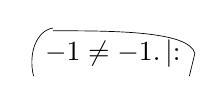
\begin{tikzpicture}
\node[inner sep=3pt] (ineq) {$-1\ne\lVert-1\rVert\unsure{\mathpunct{.}|\mathpunct{:}}$};
\draw[line width=.25pt] ([xshift=-1pt]ineq.south west) .. controls ([xshift=-3pt]ineq.west) and (ineq.north west) .. ([xshift=6pt,yshift=1pt]ineq.north west);
\draw[line width=.25pt] ([xshift=6pt]ineq.north west) .. controls (ineq.north) and (ineq.north east) .. ([xshift=2pt]ineq.east) -- (ineq.south east);
\end{tikzpicture}}
% archive sheet number: 3
\clearpage

\scanpage{5}
\[
L_{\unsure{v|\nu}}(M\otimes T,s)=L_{\unsure{v|\nu}}(M)(s\pm1)
\]

\[
\gamma_{\mathbb{R}}(s)\,\gamma_{\mathbb{R}}(s+1)
=\gamma_{\mathbb{C}}\unsure{\mathpunct{.}|\mathpunct{:}}(s)
\]
% archive sheet number: 4
\clearpage

\scanpage{6}
\margin{\tikz[baseline=(eq.base)]{\node[inner sep=3pt] (eq) {$\dfrac{E}{Q}$};\draw[line width=.35pt] (eq.north east) .. controls ([xshift=1pt]eq.east) and (eq.south east) .. (eq.south east) -- ([xshift=-3pt]eq.south west);}}

\diagram{\begin{tikzcd}[ampersand replacement=\&,column sep=.7em,row sep=1em,
execute at end picture={
\draw[line width=.25pt] ([xshift=2pt,yshift=6pt]sa.north west) -- ([xshift=-4pt,yshift=6pt]sa.north west) .. controls (sa.west) and ([xshift=-6pt]ce.west) .. ([xshift=-6pt,yshift=-5pt]ce.south west) -- ([xshift=-1pt,yshift=-5pt]ce.south west);
\draw[line width=.25pt] ([xshift=-1pt,yshift=4pt]sa.north east) -- ([xshift=4pt,yshift=4pt]sa.north east) .. controls ([xshift=6pt]sa.east) and ([xshift=4pt]ce.east) .. ([xshift=7pt,yshift=-4pt]ce.south east) -- ([xshift=0pt,yshift=-5pt]ce.south east);
}]
\& \& \& \& \mathbb{G}_m\,\unsure{\cdot|\mathpunct{.}}\\
E^{*}\arrow[r] \&
{\dfrac{\displaystyle\prod_{E/Q}\mathbb{G}_m}{\overline{U^{\unsure{\wedge|\lambda}}}}} \&
\times \& {\dfrac{I(E)}{I^{\unsure{0|\circ}}(E)}}\arrow[r] \& S_E\arrow[u]\\[-.6em]
\& \& \& \& S_{\unsure{E|\epsilon}}(\unsure{\mathbb{C}|\mathbb{R}|\mathbb{Q}})\\[-.6em]
E^{*}\arrow[d,equal] \arrow[r] \& {\text{\uline{$I(E)$}}} \&
\times \& {\dfrac{I(E)}{I^{\unsure{0|\circ}}(E)}}\arrow[r] \& |[alias=sa]| S_E(\mathbb{A})\arrow[u]\\
E^{*}\arrow[rr] \& \& I(E)\arrow[ul,"{\unsure{2|1}}"]\arrow[ur,"{1}"']\arrow[rr] \&
\& |[alias=ce]| {\text{\uuline{$C(E)$}}}\arrow[u]
\end{tikzcd}}
\figure{\begin{tikzpicture}[x=1cm,y=1cm]
\draw[line width=.25pt] (0,0) .. controls (.5,.15) and (1.7,.17) .. (2.7,.17) .. controls (5.5,.35) and (8,.45) .. (10,.42);
\end{tikzpicture}}

\[
\deleted{S_E\longrightarrow\unsure{G|\mathbb{G}}},\qquad
S_E\longrightarrow\mathbb{G}_{m}^{\unsure{h|r_{2}|r}(\unsure{E|K})}
\]
% slanted
\margin{$\unsure{2|\mathbb{Z}}_{\unsure{ve|me|e|\infty}}$}
% archive sheet number: 5
\clearpage
